\documentclass{article}
\usepackage[utf8]{inputenc}
\usepackage{latexsym}
\usepackage{amsmath, amssymb, graphics, setspace}
\usepackage{amsmath} % Define various maths environments
\usepackage{amssymb} % Define various maths symbols
\usepackage{amsthm}
\usepackage{amscd}
\usepackage{threeparttable}
\usepackage{algpseudocode}
\usepackage{geometry} % Adjust the margin, paper size, and etc.
\usepackage{enumerate} % Provide different style of lists
\usepackage{graphicx} % Insert image of all types
\usepackage{xcolor}
\usepackage{ulem}
\usepackage{pdfpages}
\usepackage{array} % Provide auxiliary format for tabular
\usepackage{booktabs} % Create Three-line Table
\usepackage{bm}
\usepackage{url}
\usepackage{hyperref}
\usepackage{float}
\usepackage{indentfirst}
\usepackage{multirow}
\usepackage{setspace}
\usepackage{enumitem}
\usepackage{ragged2e}
\usepackage{graphicx}
\usepackage{subfigure}
\usepackage{caption}
\usepackage{autofancyhdr}
\usepackage{lastpage}
\usepackage{listings}
\usepackage{algorithm2e}
\usepackage{hyphenat}
\usepackage{subfigure} 


\title{Examining the Distribution of Green Spaces through Income Inequality}
\author{Hannah Barnard, Sadhvika Challa, Hanlin Gao, Vivian Guo}

\begin{document}

\maketitle


\section{Problem Background}

\setlength{\parindent}{0pt}

Urbanization is a growing global trend; UN World Urbanization Prospects projects that by 2050, more than two-thirds of the world will live in urban areas \cite{2}. The importance of urban greenspace increases with more and more individuals moving into densely populated areas. Research shows that urban greenspaces – including parks, greenways, green infrastructure, trees, and other open spaces – have several benefits for human health, environmental health, social connections, and economic development \cite{1}. The recent COVID-19 pandemic also reminds people of the fundamental importance of greenspaces to maintaining a healthy life \cite{3}. Therefore, access to greenspaces is vital to everyone. \\

The majority of the United States population lives in densely populated areas. While there are many parks and trees in the U.S. not everyone has equal access to those greenspaces. However, research highlights significant greenspace inequities across racial/ethnic and socioeconomic lines, especially for parks \cite{4}. This can have adverse effects on the populations that do not have this access.





\section{Topic Question}

We seek to answer a series of three questions:

\begin{enumerate}
    \item Does income inequality cause disproportionate access to greenspaces?
    \item Does lower access to greenspaces result in poor health?
    \item Does this put the poor at more of a disadvantage to improve their well-being?
\end{enumerate}

These questions examine the vicious circle between income inequality, accessibility of greenspaces, and health situations. These questions could be the basis of infrastructure reform at the federal level, as the United States continues to fight the mental and physical health crisis of lower-income populations. These questions can also impact policy reform in cities with a low-income level; there is an extreme lack of policies regarding the number of greenspaces a city should be required to have.




\section{Executive Summary}

The research question that we chose had three parts. First, does income inequality correlate to access to greenspaces? Second, does having less greenspace correlate with having a lower health standard? Third, based on the answers to the first two questions, are the poor in the United States put at an even larger disadvantage to improve their livelihoods? To answer these questions, we visualized distributions of data and applied Interquartile Range Analysis to improve the quality of our dataset. Using this analysis we were able to drop extreme outliers and null data points that allowed us to better examine the real relationship between our variables.\\

To answer the first question we plotted the tree gap percentage by county against the mean percentage of tree cover by county. By doing so we were able to find a positive correlation between the two. This shows that the more trees in a county, the higher percentage of those trees are more accessible to the higher income population of the county than the lower income population.\\

To answer the second question we plotted the number of physically unhealthy days to mean tree coverage. We found that physically unhealthy days had a direct correlation to mentally unhealthy days, with generally more mentally unhealthy days for all of the counties than physically unhealthy days. We found a slight inverse correlation between greenspace and unhealthy days; the relation was more visible when the greenspace variable was mean percent tree cover than when greenspace was restricted to public parkland.\\

Our third question extends from the analysis of our first two questions. From question 1, we found that income disparity relates to lower access to greenspaces. From the second question, we uncovered a weak inverse relationship between the number of unhealthy days and the amount of greenspace. It is evident that low-income populations are disadvantaged in greenspace access. The previous result, combined with the hinted link between greenspace and perceived unhealthy days suggests a need to actively accommodate low-income regions in greenspace development, and to further monitor the impact of greenspace on individuals’ perception of health.



\section{Technical Exposition}

\subsection{Data Collection}

\subsubsection{FIPS Codes Datasets}
FIPS Code Dataset is a dataset that maps fips codes to their respective county and states (with abbreviations) within the US. US territories are also included in this dataset. The dataset contains five columns, including state, state code, state name, county code, and county. This is a dataset we used to map different other datasets. To make it easier to identify with other datasets, we first concatenate state code with county code to create a new column named county id. Then, to make the county names uniform across our datasets, we delete the ”county” postfix in each term. We create another column named state county to map between different datasets. 



\subsubsection{Urban Tree Canopy Datasets}

Urban Tree Canopy Dataset is a dataset built to help understand tree canopy and its association with income inequality across over 5000 US cities. The dataset has eight columns, including city name, census block, mean percent tree cover, tree gap, surface gap, income percent, income group, and pop dens group. 


\begin{enumerate}
    \item City name is the name of the metropolitan area and state name concatenated into a single string. 
    \item Census block is the geoid of the corresponding census block.
    \item Mean percent tree cover is the average of the percent tree cover per census block.
    \item Tree gap is the gap in tree cover between low-income and high-income census blocks.
    \item Surface temp is the mean summer surface temperature. 
    \item Income percent is the mean household income (USD) per census block. 
    \item Income group is four quantiles per city divided by Household income (in U.S. dollars), represented by values 1-4. A household that earns less than \$25,000 per year is represented by 1, between \$25,000 to \$35,000 by 2, between \$35,000 to \$55,000 by 3 and greater than \$55,000 by 4. 
    \item Pop dens group divides counties by population density (people per square kilometer), represented by values 1-4. Population density which is less than 2000 is represented by 1, between 2000 to 4000 by 2, between 4000 to 8000 by 3 and greater than 8000 by 4. 

    
\end{enumerate}
       
City name and surface temp columns are not relevant to our study; we first drop these columns of data. Then, since we want to focus on medium to high-density urban centers, we filter the data to entries belonging to a population density group larger than or equal to 3. Post filtering, we clean our data of erroneous entries and missing entries; we ensure that income entries are non-negative and drop all entries with missing data.\\

\begin{figure}[H]
    \centering
    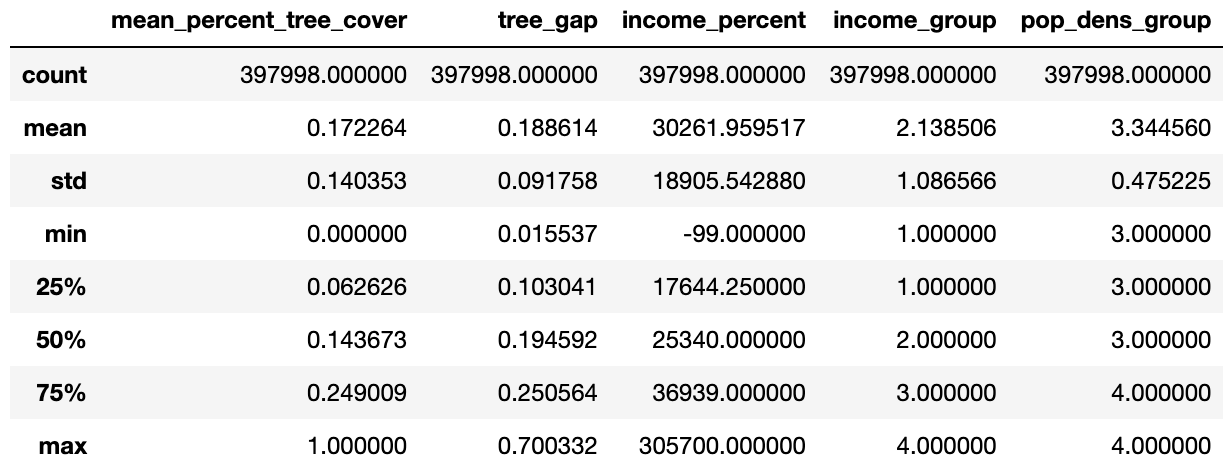
\includegraphics[scale = 0.5]{summ_urban.png}
    \caption{Summary of Urban Tree Canopy dataset to aid data cleaning process}
    \label{fig:my_label}
\end{figure}

Then, we shift focus to reducing outliers to minimize mistakes of our dataset and thereby increase the strength of our analysis.


\begin{figure}[H]
    \centering
    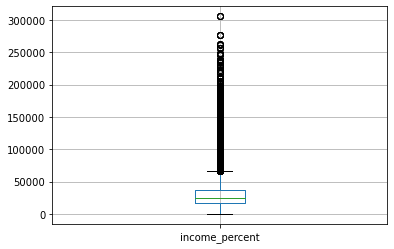
\includegraphics[scale = 0.5]{income_percent_box_plot.png}
    \caption{Box plot of income percent}
    \label{fig:my_label}
\end{figure}

From the box plot of income percent, we observe that a significant portion of data would be outliers if we apply interquartile range (IQR) analysis for outlier reduction. This could result from existing income inequality in the dataset. In 2010, the US scored 0.469 on the Gini Index, an index of income inequality \cite{6}. We chose not to apply IQR to income.


\begin{figure}[H]
    \centering
    \subfigure[Mean tree cover box plot before]{
    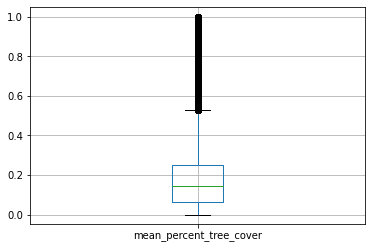
\includegraphics[scale = 0.35]{mean_tree_cover_box_plot_before.png}
    }
    \quad
    \subfigure[Mean tree cover box plot after]{
    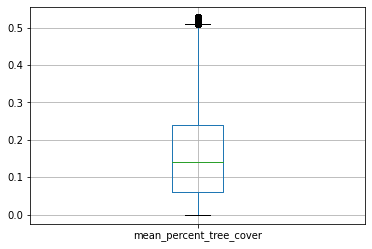
\includegraphics[scale = 0.35]{mean_tree_cover_box_plot_after.png}
    }
    \quad
    \subfigure[Tree gap box plot before]{
    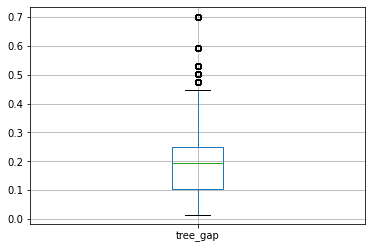
\includegraphics[scale = 0.35]{tree_gap_box_plot_before.png}
    }
    \quad\subfigure[Tree gap box plot after]{
    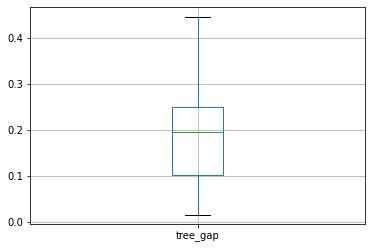
\includegraphics[scale = 0.35]{tree_gap_box_plot_after.png}
    }
    \caption{Box plot of mean tree cover and tree gap before and after deleting outliers}
    \label{fig:my_label}
\end{figure}

We perform IQR outlier reduction on each mean tree cover data and tree gap data and create box plots to visualize the effectiveness of the reduction. 
 \\

To further analyze the data, we visualize density plots for income percent, tree gap and mean tree cover.


\begin{figure}[H]
    \centering
    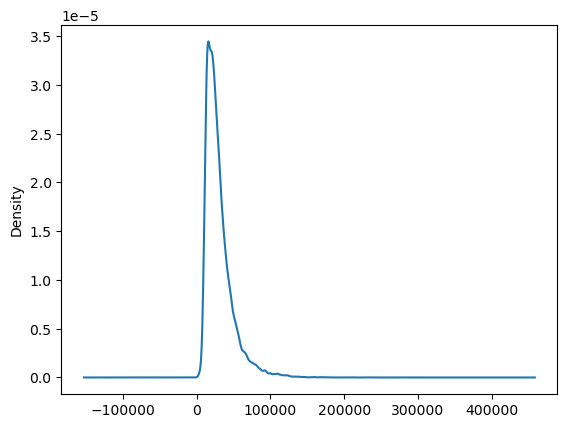
\includegraphics[scale = 0.4]{income_percent_density.png}
    \caption{Income percent density}
    \label{fig:my_label}
\end{figure}

\begin{figure}[H]
    \centering
    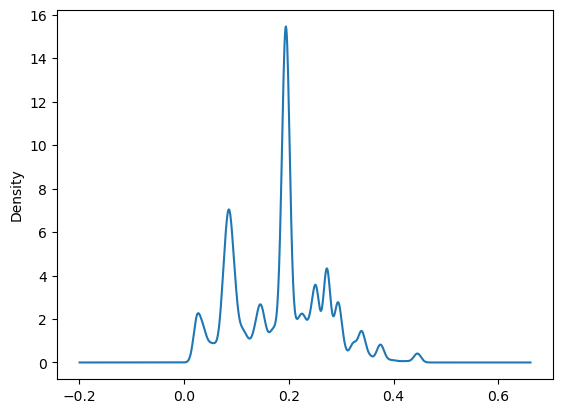
\includegraphics[scale = 0.4]{tree_gap_density.png}
    \caption{Tree gap density}
    \label{fig:my_label}
\end{figure}

\begin{figure}[H]
    \centering
    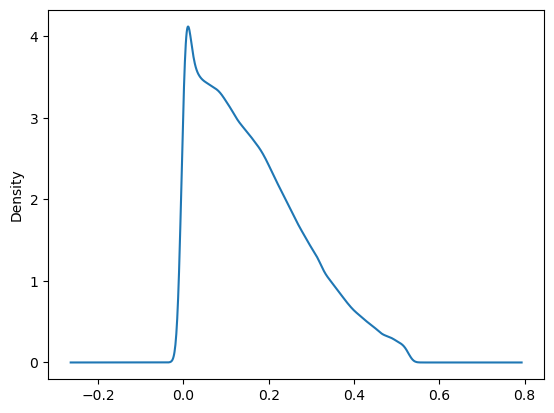
\includegraphics[scale = 0.4]{mean_percent_cover_density.png}
    \caption{Mean tree cover density}
    \label{fig:my_label}
\end{figure}

From the graphs above, we observe that the income percent and mean tree cover data have a right skew distribution, while the tree gap data’s distribution is relatively symmetrical. We also calculated the skewness and kurtosis for each data type. The calculated results are shown in the following table. For income percent data, the skewness is positive and thus more weight is in the left tail of the distribution. Additionally, the kurtosis is larger than 3, which signifies that it tries to produce more outliers rather than the normal distribution. It also accords with our previous analysis that there are far too many outliers for the income percent data. For the tree gap data, the skewness is positive, but minor, which means there is more weight in the left tail of the distribution. For mean tree cover, the skewness is also positive and minor, which means there is more weight in the left tail of the distribution. The kurtosis of both tree gap and mean tree cover are less than 3, which accords with our previous boxplots. 



\begin{table}[h!]
\centering
\begin{tabular}{|c |c c c|} 
 \hline
  & Income Percent & Tree Gap & Mean Tree Cover \\ [0.5ex] 
 \hline
 Skewness & 2.373856 & 0.440392 & 0.724803 \\ 
 Kurtosis & 10.376055 & 0.475697 & -0.184217 \\
 \hline
\end{tabular}
\caption{Skewness and Kurtosis Analysis}
\label{table:1}
\end{table}


\subsubsection{2010 National Health Datasets}
The health data set that was given was not from the same year as the other census data, so it was not ideal for comparison. That data set was also supplied by mental health institutions, which would mean we would only be looking at data from individuals who had access to those services. This would have added unnecessary bias to our data. \\

Therefore, we searched for different health data that would be more useful to our research question. Countyhealthrankings.org is a program created by the University of Wisconsin Population Health Institute. They consolidate data from the American Medical Association, Community Partnerships for Health Equity (CPHE-MEDICC), and other vetted sources to help give access to important health data to the public. This record holds county health data from 2010. We obtained health data by county and it is stored inside of “2010nationalhealth.csv” \cite{5}. This data allowed us to see health discrepancies among counties in the same year as the rest of our data. \\

We focused on the poor physical and mental health days of this dataset, which measures individuals’ perception of their physical and mental health by reporting the number of unhealthy days one experiences in a month.\\

The poor physical health days data contains 5 columns, including sample size (number of respondents between 2002 and 2008), physically unhealthy days (average number of reported physically unhealthy days per month), 95\% CI - Low and 95\% CI - High (95\% confidence interval reported by BRFSS, and Quartile (Within-state rank: 1 = top quartile, 2=second quartile, 3= third quartile, 4=bottom quartile). \\

Similarly, the poor mental health days data contains 5 columns, including sample size (number of respondents between 2002 and 2008), physically unhealthy days (average number of reported mentally unhealthy days per month), 95\% CI - Low and 95\% CI - High (95\% confidence interval reported by BRFSS, and Quartile (Within-state rank: 1 = top quartile, 2=second quartile, 3= third quartile, 4=bottom quartile). \\

We first delete all of the columns and rows without any data entry. Then, we create a new column of county id and map it with FIPS data to allow for comparison with other datasets.


\subsubsection{Percent Cover County Datasets}
The percent cover county dataset is a dataset of the percent park cover per GEOID across the US at an aggregation of a specific county. It contains three columns, including GEOID (concatenation of various FIP codes used by the US Census Bureau to identify different levels of hierarchy in geographic organization), county name, and percent of land for a GEOID that is public accessible parkland. We read the dataset from the txt file and drop the unuseful county name column, all empty data entries, and duplicated GEOIDs. Our clean dataset consists of a column representing GEOID and another representing the percent of land that is public accessible parkland for each GEOID.



\subsection{Exploratory Data Analysis}
We seek to find a relation between income inequality and the creation of greenspaces, then between the quantity of greenspace and individual health. Post data cleaning, our study is across 359 densely populated counties. With much of our data normalized, we apply linear regression to observe relationships. To begin our analysis, we explore the common link of greenspace data.


\subsubsection{Distribution of Public Accessible Parkland by County}

Below shows the distribution of the percent public accessible parkland across our dataset. Most counties have less than 20\% of public accessible parkland. Given the importance of urban greenspace, this indicates a national need for the expansion of greenspace infrastructure regardless of income inequality. 


\begin{figure}[H]
    \centering
    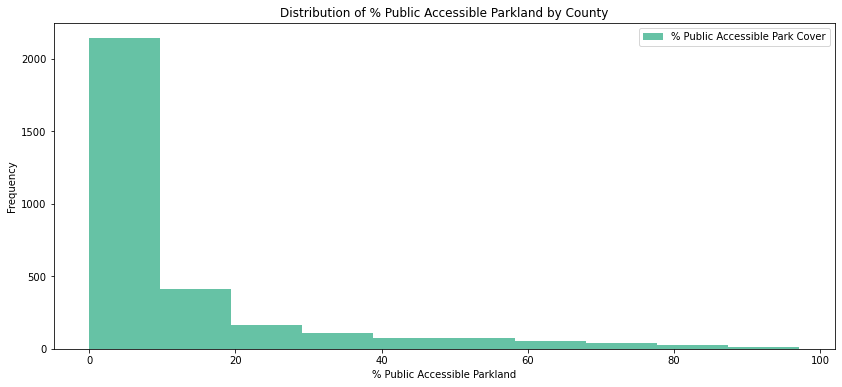
\includegraphics[scale = 0.4]{park.png}
    \caption{Distribution of \% Public Accessible Parkland by County}
    \label{fig:my_label}
\end{figure}

\subsubsection{Mean Percent Tree Cover and Tree Gap by County}
We sort county IDs by mean percent tree cover in ascending order to search for a connection between the mean percent tree cover and tree cover gap from income inequality. The linear regression model for tree cover gap depicts an upward trend as the mean percent tree cover increases. This suggests in counties with more tree cover, areas of higher income have better access to the added tree cover. The disproportionate tree cover access between low and high-income areas prompts a need for policymakers to consciously accommodate low-income areas when investing in urban greenspaces.

\begin{figure}[H]
    \centering
    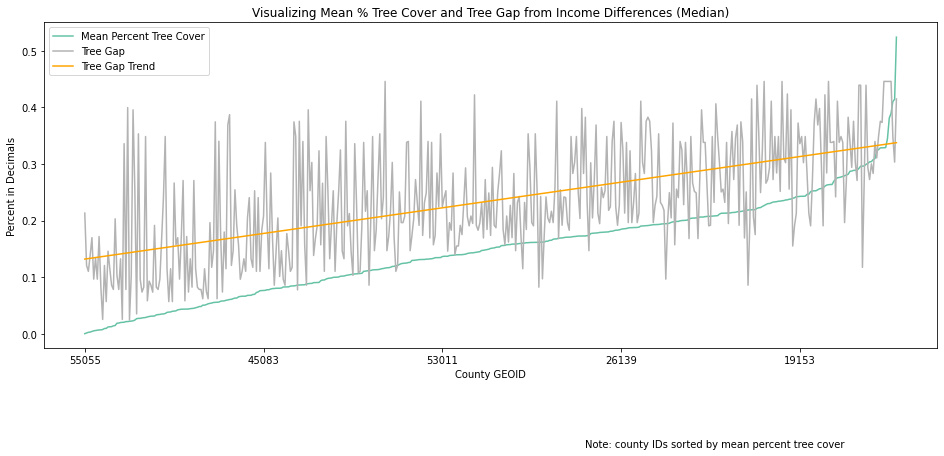
\includegraphics[scale = 0.4]{mean_pecent_tree_cover_tree_gap.png}
    \caption{Visualizing Mean Percent Tree Cover and Tree Gap from Income Differences (Median)}
    \label{fig:my_label}
\end{figure}

\subsubsection{Unhealthy Days}
We explore the relationship between an individual’s health with income, mean percent tree cover, tree cover gap, then accessible parkland. Each dataset is sorted by physically unhealthy days (PUD) or mentally unhealthy days (MUD), with unhealthy days normalized between 0 to 1. 

\setcounter{secnumdepth}{4}
\paragraph{Average House Hold Income}

The visualization below shows an inverse relationship between unhealthy days and average household income. As the reported number of PUDs increase, the average household income decreases. This suggests lower income individuals feel more physically unhealthy. We see a similar result when comparing income and MUD in those counties with lower average household income who feel more mentally unhealthy.



\begin{figure}[H]
    \centering
    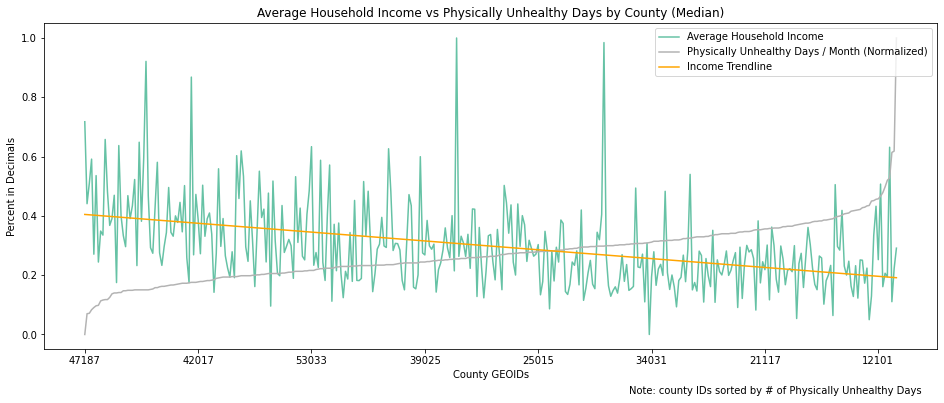
\includegraphics[scale = 0.4]{avg_income_phys.png}
    \caption{Average Household Income vs Physically Unhealthy Days by County (Median)}
    \label{fig:my_label}
\end{figure}

\begin{figure}[H]
    \centering
    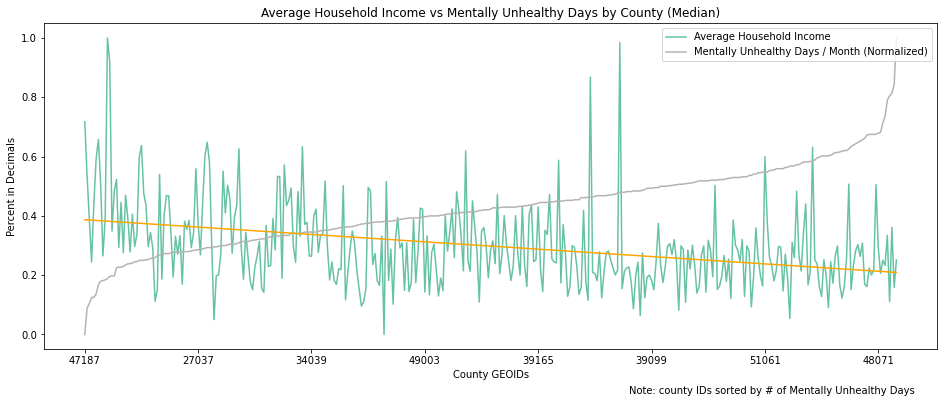
\includegraphics[scale = 0.4]{avg_income_mental.png}
    \caption{Average Household Income vs Physically Unhealthy Days by County (Median)}
    \label{fig:my_label}
\end{figure}

\paragraph{Mean Percent Tree Cover}
Through linear regression models of unhealthy days with mean percent tree cover, there is an observable negative relation where the increase of mean percent tree cover relates to lower unhealthy days. With mean percent tree cover as the independent variable, we compare both types of unhealthy days and note that people tend to report a higher number of MUDs than PUDs. Mean percent tree cover appears to have a greater impact on MUDs as opposed to PUDs. Whereas the PUD trendline of normalized values ranges from 25.1\% to 29.4\% with a difference of 4.27\%, the MUD trendline’s values range from 39.8\% to 45.5\% with a difference of 5.71\%.



\begin{figure}[H]
    \centering
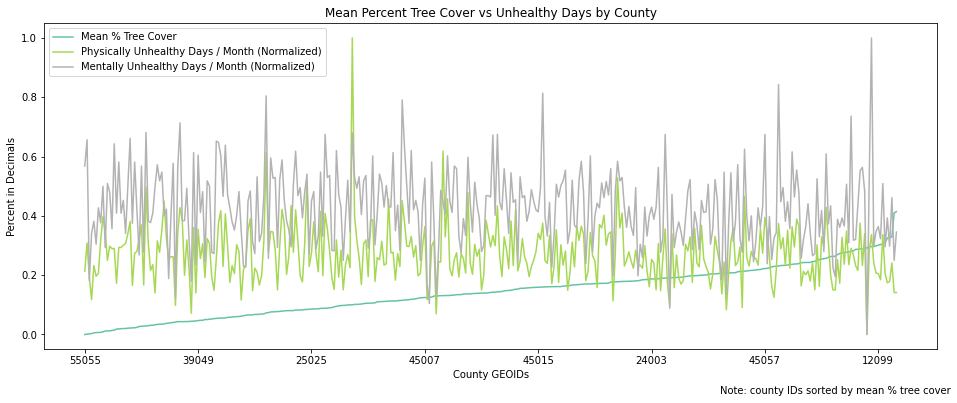
\includegraphics[scale = 0.4]{mean_percent_tree_cover_phys_ment.png}
    \caption{Mean Percent Tree Cover vs Unhealthy Days by County}
    \label{fig:my_label}
\end{figure}

\begin{figure}[H]
    \centering
    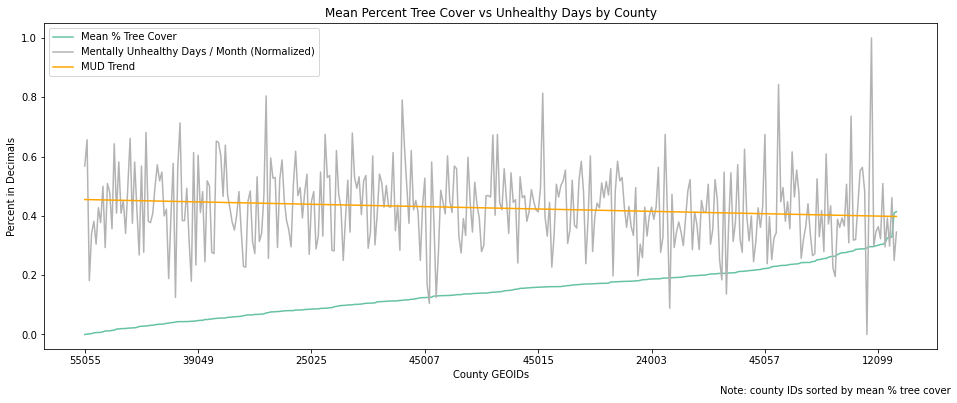
\includegraphics[scale = 0.4]{mean_percent_unhealth.png}
    \caption{Mean Percent Tree Cover vs Mentally Unhealthy Days by County}
    \label{fig:my_label}
\end{figure}


\begin{figure}[H]
    \centering
    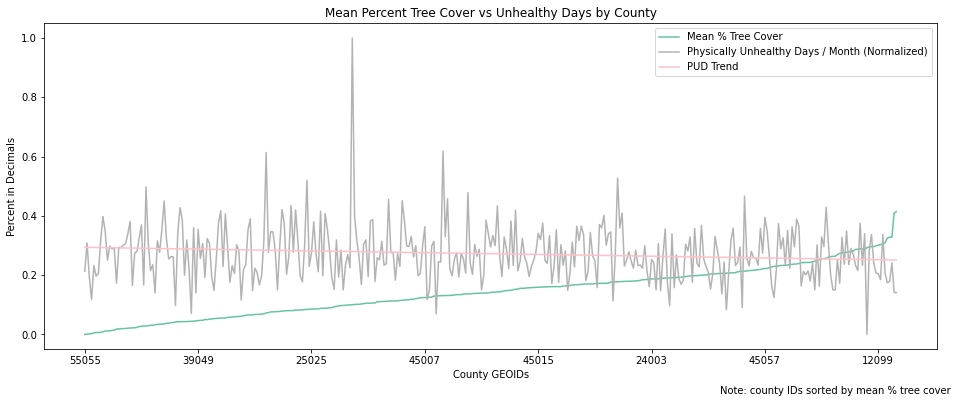
\includegraphics[scale = 0.4]{mean_percent_unhealth_ment.png}
    \caption{Mean Percent Tree Cover vs Physically Unhealthy Days by County}
    \label{fig:my_label}
\end{figure}

\paragraph{Public Accessible Park Cover}
When comparing percent public accessible parkland with unhealthy days, there is a very slight relation where a rise in the percentage of publicly accessible parkland in a county relates to less both PUDs and MUDs. The variation for the PUD trendline has a range of 1.42\% while the MUD trendline has a range of 1.82\%. This relation is weaker than that of the mean percent tree cover to unhealthy days, which suggests the presence of general greenspace in an area impacts individuals more than its accessibility. 


\begin{figure}[H]
    \centering
    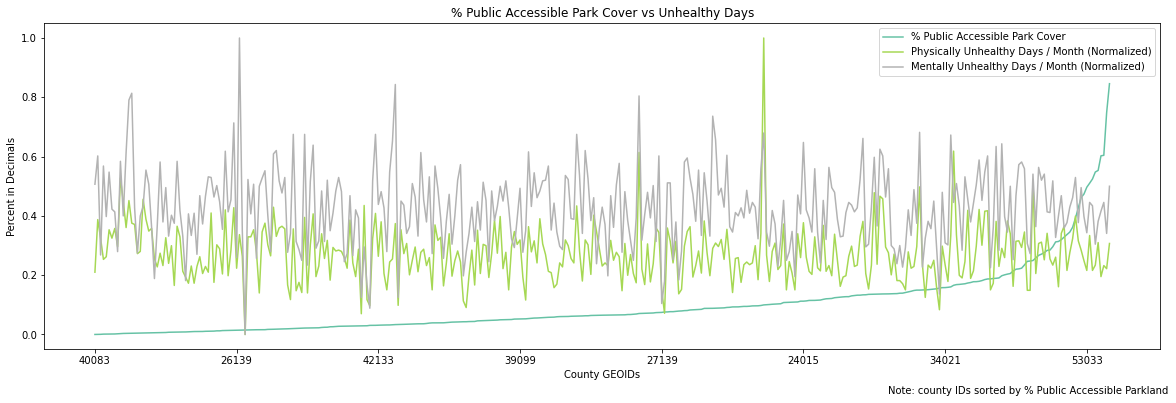
\includegraphics[scale = 0.35]{park_phys_ment.png}
    \caption{Public Accessible Park Cover vs Unhealthy Days}
    \label{fig:my_label}
\end{figure}




\begin{figure}[H]
    \centering
    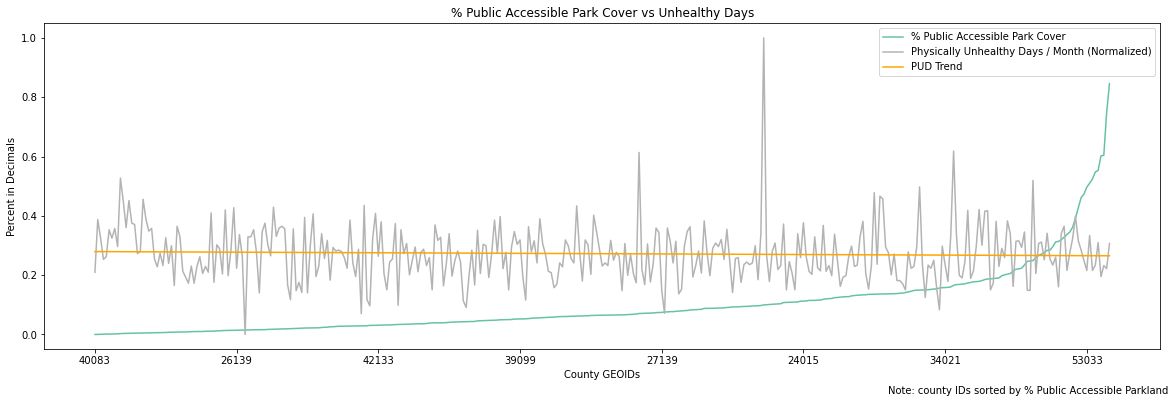
\includegraphics[scale = 0.35]{park_cover_phys.png}
    \caption{Public Accessible Park Cover vs Mentally Unhealthy Days}
    \label{fig:my_label}
\end{figure}



\begin{figure}[H]
    \centering
    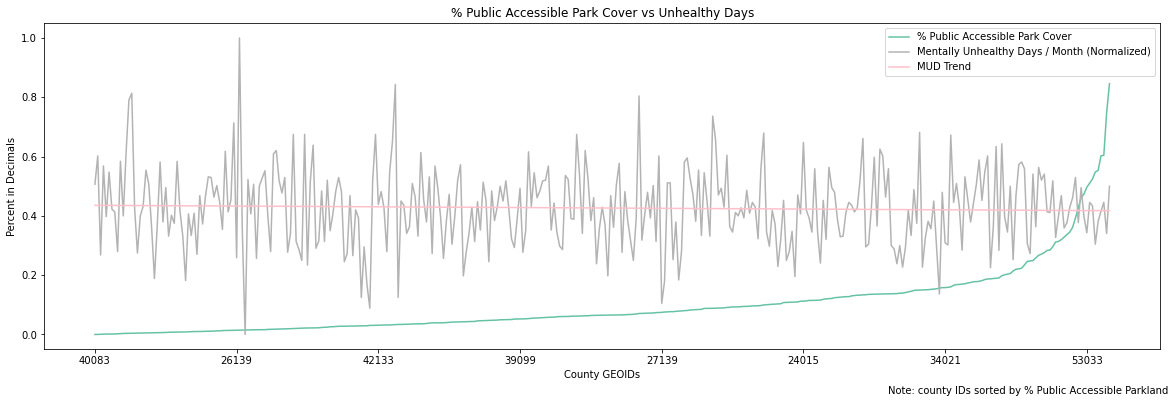
\includegraphics[scale = 0.35]{park_cover_ment.png}
    \caption{Public Accessible Park Cover vs Mentally Unhealthy Days}
    \label{fig:my_label}
\end{figure}



\subsection{Discussion and Conclusion}
Our study explores greenspace access with income inequality, as well as how disproportionate green space access may perpetuate income inequality due to relations between health and greenspace. \\

The results indicate an existing greenspace access issue, where wealthier communities in counties have better access than lower-income communities. As well, increases in greenspace add to wealthier individuals’ access more than others. The further this trend continues, the more difficult and costly it will be to balance greenspace access between varying income groups. With regards to the population’s perceived unhealthy days, there is a weak, but observable association of better-perceived health from lower unhealthy day counts with more greenspace. Moreover, individuals’ mental health perception appears more sensitive to greenspace access than physical health perception. With the notable correlation between more unhealthy days and less income in mind, disproportionate greenspace access due to income inequality is one that policymakers should address to improve the well-being of growing urban communities. 


\newpage

\begin{thebibliography}{9}
\bibitem{2}

Hannah Ritchie and Max Roser (2018) - "Urbanization". Published online at OurWorldInData.org. Retrieved from: 'https://ourworldindata.org/urbanization' [Online Resource]

\bibitem{1}
Crompton, J. L., \& Nicholls, S. (2020). Impact on property values of distance to parks and open spaces: An update of US studies in the new millennium. Journal of Leisure Research, 51(2), 127-146.



\bibitem{3}
Kleinschroth, F., \& Kowarik, I. (2020). COVID‐19 crisis demonstrates the urgent need for urban greenspaces. Frontiers in Ecology and the Environment, 18(6), 318. 

\bibitem{4}
Koprowska, K. (2019). Environmental justice in the context of urban green space availability. Acta Universitatis Lodziensis. Folia Oeconomica, 6(345), 141-161.

\bibitem{5}
Rankings Data \&amp; Documentation: National Data \&amp; Documentation: 2010-2020. County Health Rankings \&amp; Roadmaps. (n.d.). Retrieved February 12, 2023, from https://www.countyhealthrankings.org/explore-health-rankings/rankings-data-documentation/national-data-documentation-2010-2019 [Online Resource]

\bibitem{6}
U.S. Census Bureau (2011). “Income, Poverty and Health Insurance Coverage in the United States: 2010”. Retrieved from https://www.census.gov/newsroom/releases/archives/income\_wealth/ [Online Resource]




\end{thebibliography}

\end{document}
